\documentclass[conference]{IEEEtran}


  	\usepackage[pdftex]{graphicx}
  	\graphicspath{{../pdf/}{../jpeg/}}
	\DeclareGraphicsExtensions{.pdf,.jpeg,.png}

	\usepackage[cmex10]{amsmath}
	\usepackage{mathabx}
	\usepackage{algorithmic}
	\usepackage{array}
	\usepackage{mdwmath}
	\usepackage{mdwtab}
	\usepackage{eqparbox}
	\usepackage{url}
	\hyphenation{op-tical net-works semi-conduc-tor}


\begin{document}

\title{\LARGE PWM Techniques For Parallel Connected Voltage Source Inverters}

% \author{\authorblockN{Leave Author List blank for your IMS2013 Summary (initial) submission.\\ IMS2013 will be rigorously enforcing the new double-blind reviewing requirements.}
% \authorblockA{\authorrefmark{1}Leave Affiliation List blank for your Summary (initial) submission}}

 \author{\authorblockN{Aashish Bhorse(2015EE30501), Abhay Singh(2015EE30502) }}
 

\maketitle

\begin{abstract}
In this report we have done analysis of different type of Pulse-width Modulation(PWM) technique for the two interleaved, three phase, two level Voltage source inverters. We have analyzed that the behavior of circulating current for different PWM methods. Circulating current is not depended on the load current rather its depends on the difference between common mode voltages of the two interleaved voltage source inverters, angle of interleaved and the method of PWM which is used. we have also analyzed THD(Total Harmonic Distortion) in load side phase current for different PWM technique.
\end{abstract}

\IEEEoverridecommandlockouts
\begin{keywords}
Pulse-width Modulation, circulating current, Harmonic Distortion, Space vector.
\end{keywords}

\IEEEpeerreviewmaketitle


% ===================
% # I. Introduction #
% ===================

\section{Introduction}
Voltage source inverters are used in the variety of applications where we need dc-ac energy conversation. VSI generates low frequency output voltage with controllable magnitude and frequency with the help of high frequency voltage signals or pulses. The harmonic distortion of the line current of the voltage source inverter must be low for the satisfactory operation for any applications like induction motor drive. 

Parallel connected voltage source inverters have many advantage of single VSI. The main  advantages are reduced current stress in the switching devises, improve in the thermal management, reduction in current ripple, increased in power capability, easy maintenance and increase in efficiency. Parallel interleaved VSIs have a common dc link, their carrier signals are interleaved(i.e. the two signals are phase shifted) and their ac side is connected through an inductive coils.

Due to a common dc link their is an circulating current which flows in between the two interleaved VSIs and due to this circulating current losses occurs in the switching devices. The circulating current is depends on the angle of interleave and the method of PWM which is used. The main cause of circulating current is common mode voltage difference if two VSLs and which depends on interleave angle. If we keep interleave angle equal to zero then their will not be any circulating current but at the same condition the line current or ac side current will contain more harmonics distortion or we can say that ac side current will have more rms ripple current. That's why we want to optimize the PWM methods with interleave angle such that ac side current has less harmonic distortion and less circulating current between the interleaved VSIs.

% =======================================================
% # II. Impact of traps on large signal characteristics #
% =======================================================

\section{Conventional PWM Techniques}
 Sinusoidal PWM method is the simplest and easy in implementation. In SPWM the reference wave is sine wave signal which is compared with a high frequency triangular carrier signal and it's intersection defines the switching instances. Adding an offset to the reference sine wave leads to produced different characteristics of the circulating current and ac side line current. In Space vector PWM, space vector theory is used in which an reference signal is rotating a 2D plane.
 In the SVPWM method dq transformation has done using voltage-second balance theory and an voltage vector is generated which is equivalence to the reference voltage signal. The 360 degree space is divided into 6 equal sectors and in every sector the nearest voltage vectors(in which two are active vectors and two are zero vectors) are used to generate the reference voltage vector. 
 
 The main difference in all of the PWM methods is how we used two zero voltage vectors along with the two nearest voltage vector to the reference voltage vector or we can say the how we use switching sequence to generate the desired output voltage. In the SVPWM technique both of the zero voltage vector is used for equal time in a particular sub-cycle.
\section{Simulation Results}


\begin{figure}[ht!] %!t
\centering
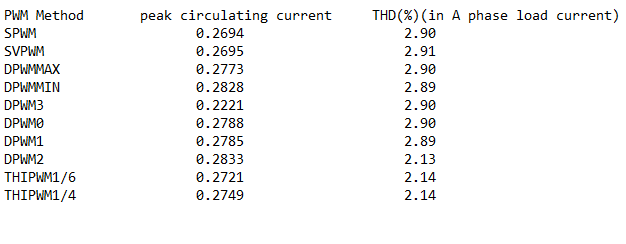
\includegraphics[width=3.5in]{Result.PNG}}
\caption{Peak circulating current and THD in ac side current for different PWM Methods at m=0.8}
\label{Courant_2}
\end{figure}


% ==================
% # IV. CONCLUSION #
% ==================

\section{Conclusion}
From the simulation result we can see that for DPWM3 method we are getting minimum circulating current but THD in ac side current is high and for DPWM2 method we are getting minimum THD in ac side current but peak circulating current is pretty high. So, as we are trying to decrease circulating current, the THD in ac side current is increases and vice versa, so, circulating current and THD in ac side current contradict each other. So, we want to set a trade off between circulating current and THD in ac side current such that we can get both minimum.




% ==================
% # ACKNOLEDGMENTS #
% ==================

% use section* for acknowledgement
%\section*{Acknowledgment}
% The authors would like to thank...


% ==============
% # REFERENCES #
% ==============
\section{References}
[1] Kapil Shukla , Varun Malyala, and Ramkrishan Maheshwari” A novel carrier based hybrid PWM technique for minimization of line current ripple in two interleaved two-level VSIs” 

[2] Ramkrishan Maheshwari, Ghanshyamsinh Gohil, Lorand Bede, Stig Munk-Nielsen” Analysis and Modeling of circulating current in two parallel-connected inveters” 

\bibliographystyle{IEEEtran}
\bibliography{IEEEabrv,biblio_traps_dynamics}
 
\end{document}

